\documentclass[conference]{IEEEtran}
\IEEEoverridecommandlockouts
% The preceding line is only needed to identify funding in the first footnote. If that is unneeded, please comment it out.
\usepackage{cite}
\usepackage{amsmath,amssymb,amsfonts}
\usepackage{algorithmic}
\usepackage{algorithm}
\renewcommand{\algorithmicrequire}{ \textbf{Input:}} %Use Input in the format of Algorithm
\renewcommand{\algorithmicensure}{ \textbf{Output:}} %UseOutput in the format of Algorithm
\usepackage{graphicx}
\usepackage{graphicx}
\usepackage{textcomp}
\usepackage{xcolor}
\usepackage{enumerate}
\def\BibTeX{{\rm B\kern-.05em{\sc i\kern-.025em b}\kern-.08em
    T\kern-.1667em\lower.7ex\hbox{E}\kern-.125emX}}
\begin{document}

\title{GaoNing}

\author{\IEEEauthorblockN{1\textsuperscript{st} Given Name Surname}
\IEEEauthorblockA{\textit{dept. name of organization (of Aff.)} \\
\textit{name of organization (of Aff.)}\\
City, Country \\
email address}
\and
\IEEEauthorblockN{2\textsuperscript{nd} Given Name Surname}
\IEEEauthorblockA{\textit{dept. name of organization (of Aff.)} \\
\textit{name of organization (of Aff.)}\\
City, Country \\
email address}
\and
\IEEEauthorblockN{3\textsuperscript{rd} Given Name Surname}
\IEEEauthorblockA{\textit{dept. name of organization (of Aff.)} \\
\textit{name of organization (of Aff.)}\\
City, Country \\
email address}
\and
\IEEEauthorblockN{4\textsuperscript{th} Given Name Surname}
\IEEEauthorblockA{\textit{dept. name of organization (of Aff.)} \\
\textit{name of organization (of Aff.)}\\
City, Country \\
email address}
\and
\IEEEauthorblockN{5\textsuperscript{th} Given Name Surname}
\IEEEauthorblockA{\textit{dept. name of organization (of Aff.)} \\
\textit{name of organization (of Aff.)}\\
City, Country \\
email address}
\and
\IEEEauthorblockN{6\textsuperscript{th} Given Name Surname}
\IEEEauthorblockA{\textit{dept. name of organization (of Aff.)} \\
\textit{name of organization (of Aff.)}\\
City, Country \\
email address}
}

\maketitle

\begin{abstract}
This document is a model and instructions for \LaTeX.
This and the IEEEtran.cls file define the components of your paper [title, text, heads, etc.]. *CRITICAL: Do Not Use Symbols, Special Characters, Footnotes,
or Math in Paper Title or Abstract.
\end{abstract}

\begin{IEEEkeywords}
component, formatting, style, styling, insert
\end{IEEEkeywords}

\section{Introduction}
With the development of mobile Internet, a large number of new network services and applications are widely applied, such as AR/VR, mobile high definition video, online game etc., which require that the mobile network provides the higher data tra,nsmission rate and lower network delay. Moreover, it is predicted that by year 2020, the mobile data traffic will reach 30.6 exabytes/month globally\cite{cisco}. To handle the severe challenge, densely deployed small cell network (SCN) have been widely introduced by network operators to enhance the network capacity. However, the costly and heavily-loaded backhaul link between SCN and the core network is becoming the bottleneck. 

Caching on the SCN has been widely recognized as an effective and eonomical solution to tackle the aforementioned problem of network densification. By storing popular files in the SBS cache in advance\cite{6600983,6933434}, more requests can be satisfied at SBSs instead of retrieving duplicated file over the backhaul links. Besides, downloading directly from SBSs reduces download delay substantially due to the short transmission distance and thus high rate. However, the storage capacity on SBSs is generally limited, and thus caching strategies should be carefully designed to make the best use of the SBS cache.

There have been some recent works focusing on designing file caching strategies in the scenario of network densification. Reference \cite{6600983} present a wireless distributed caching stratrgy with a low-bandwidth backhaul link but high storagr capacity where user can access multiple SBSs. Finding the optimal cache placement to maximize cache hit ratio is proved to be NP complete. The authors of \cite{6600983} study the optimization issue for cache content placement in caching enabled SCN with heterogeneous file and cache sizes, and adopt multicast transmission to minimize the average backhaul rate. In [Energy-efficient Cooperative Coded Caching for Heterogeneous Small Cell Networks], the authors propose an cooperative caching strategy with a low-bandwidth backhaul link but high storagr capacity where user can access multiple SBSs. Finding the optimal cache placement to maximize cache hit ratio is proved to be NP complete. The authors of [cluster hetnet coded] study the optimization issue for cache content placement in caching enabled SCN with heterogeneous file and cache sizes, and adopt multicast transmission to minimize the average backhaul rate. In \cite{8116421}, the authors propose an cooperative caching strategy where SBS can get desired content from neighbouring SBSs so as to enhance the content delivery efficiency.

Although these recent works have provided insight into caching strategy in cellular network, users are assumed to be static and the association between users and SBSs remains unchanged. Obviously, such assumption is unreasonable. Users are mobile and the association to SBSs can change during the download of a file, which can be more   frequently with densely deployed SBSs. Therefore the impact of user mobility can not be neglect when designing file caching strategies\cite{7537180}. Reference\cite{6620380} assumes that the user movement obeys a discrete Markov model and the amount of data downloaded by users depends on their location and the cache placement in each time slot. The author of \cite{8013789}uses a descrete random jump model to describe the mobility pattern and derive the expression of throughput. Due to the complexity of the problem, two heuristic algorithms are provided to obtain the optimal solution. Reference \cite{7484297} model user mobility as Markov chain and put for forward a distributed caching paradigm in a two-tier heterogeneous network with the aim of minimizing the content fetching from MBS.

Although these works have taken user mobility into consideration, they all consider a static global file popularity among all the SBSs. The effect of mobility on content popularity at different SBSs are not well investigated. In a real system, SBSs covering different areas generally have different file popularity, considering the global popularity is not siutable. Moreover, file popularity of neighboring SBS will affect each other, because moving user may request the same file again in another SBS if he fails to complete the download in the current SBS.

In this paper, we propose a mobility-aware coordinate proavtive caching strategy. Taking advantages of heterogeneous small cell network architecture, both MBS and SBS are equipped with cache and files can be deliverd between them. In order to measure the data rate and transmission delay of the user request file together, we adopt the effective capacity criterion. Effective capacity is proposed to form channel model in link layer to calculate the data rate for a specific user with the impact of transmission delay.

The contributions of this paper include:
\begin{itemize}
 \item Allowing multiple V-UEs share the same RBs to explore the potential to accommodate more V-UEs.
 \item We construct the conflict graph based on the worst-case Signal-to-Interference Ratio(SINR).
 \item We model the allocation problem as \emph{Graph Coloring Problem}, which is NP-Complete.
 \item A Resource Sharing and Admission Control(RSAC) scheme is proposed to solve the problem.
\end{itemize}

 The remainder of this paper is organized as follows. Section II describes the system model, including network model, file popularity model, mobility model and transmission delay model. In Section III, we introduce the proposed mobility-aware coordinate proavite caching strategy and fromulate the cache placement problem as an optimization problem. In Section IV, a genetic algorithm is adopted to solve the problem. In Section V, numerical results are illustrated with performance comparisons between MPC. Finally, conclusions are summarized in Section VI.
\section{System Model}
\subsection{Network Model}
In this paper, we\cite{8116421} consider a heterogeneous network comprising a single MBS and K densely deployed SBS denoted as
$\mathbf{S} \triangleq\{1\mathrm{,\,}2\mathrm{,\,}3...\mathrm{,\,}K\}$, where $S_k$ represents the MBS. The MBS and SBSs are connected by a fronthaul link with limited capacity of $ r_{FH}$ and the MBS is connected to the EPC network by a backhaul link with limited capacity of $ r_{BH}$. The set of active users is $\mathbf{U} \triangleq\{1\mathrm{,\,}2\mathrm{,\,}3...\mathrm{,\,}U\}$ and each user only requests one file at a time while moving from one cell to another from time to time. We consider that each user u only connects to and receives data from the nearst BS (in terms of signal strength), which we later refer to as the user \emph{u’s} home BS. And the users set associate with SBS $S_k$ is denoted as $U_k$.
\begin{figure}[htbp]
 \centerline{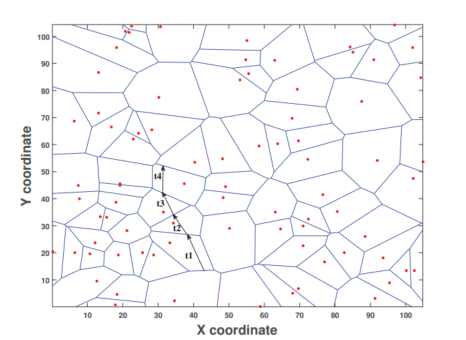
\includegraphics[scale=0.7]{fig1.png}}
 \caption{System Model.}
 \label{fig 1}
\end{figure}

We assume that the MBS has access to a library of $\mathrm{N}$ files denoted as $\mathbf{F} \triangleq\{1\mathrm{,\,}2\mathrm{,\,}3...\mathrm{,\,}N\}$, and each file has the same size denoted by $B$[MB]. Note that the assumption of equal size files is justifiable in practice since files can be divided into blocks of the same size.

We assume that SBS $S_k$ are equipped whih a cache to storage files with storage capacity of $C_i$[MB], and the MBS is equipped with a large cache with storage capacity of
$C_0 [MB]$. Each user requesting for files in $\mathbf{F}$ is initially served by the SBS he contacts. If the requested file is not present in the cache, other SBSs nearby or the MBS will send the file to the user as shown in Fig.1. To describe the cache placement decision, we define the cache placement matrix as:
$$\mathbf{X}=
\begin{Bmatrix}
x_{0,1}    &x_{0,2}  & \cdots & x_{0,N} \\
x_{1,1}    &x_{1,2}  & \cdots & x_{1,N} \\
\vdots    &\vdots  & \ddots &\vdots \\
x_{K,1}    &x_{K,2}  & \cdots & x_{K,N}
\end{Bmatrix}
$$
where $x_(i,j)$ denotes caching the file $f_j$ in $BS i$. The cache storage capacity constraints can be expressed as:

\begin{equation}
\sum_{j=1}^N B\cdot x_{[i,j]}, \quad \forall{S_i}\in\mathbf{S}
\end{equation}
\subsection{Content Populary}
We define the populary distribution of files in cell $i$ as $\mathbf{P} \triangleq\{p_{i,1}\mathrm{,\,}p_{i,2}\mathrm{,\,}p_{i,3}...\mathrm{,\,}p_{i,N}\}$, in which $p_{i,j}$ is the probability of the file $f_j$ being requested from a user in cell $i$, and $ \sum_{j=1}^N p_{i,j}=1,\,\forall{S_i}\in\mathbf{S}$.It should be noted that the content populary here is inferred with historical data and can can not reflect the short-term variation due to user mobility.
\subsection{Mobility Model}
User mobility is modeled by discrete random jumps, with the corresponding intensity characterized by average sojourn time. In terms of the distribution of sojourn time, it is reasonable to model it by an exponential function [MEC]. Therefore, the probability density function (PDF) of sojourn time in cell $i$ can be written as follows:
\begin{equation}
p(\tau,u_i)=\frac{1}{\mu_i}e^{-\tau/\mu_i},\quad \forall{S_i}\in\mathbf{S}
\end{equation}

where $\mu_i$ is the average sojourn time. Different cells have different $\mu_i$ because the coverage area of different cells is different.

In addition, in order to describe the trajectory of moving users, we adopt the stationary Markov model. Let $T_{l,i}\ge 0$ denote the probability of transition from cell $l$ to cell $i$, where $\sum_{i\in\mathbf{S}}$. When a user has incomplete download at one cell and enters the new cell, the content is requested at the new cell thus affecting the static content popularity $p_(i,j)$.Therefore, the popularity $p_(i,j)$ of content $j$ in BS $i$ may not reflect the actual request probability of content $j $in BS $i$. If the content requested by user is not cached in the new cell, it has to be fetched from EPC network via high latency link. In order to provide a better QoS service, we need to dynamically adjust the distribution of file popularity based on the user's mobile pattern, thereby reducing the huge latency caused by cache misses.
\subsection{Delay and EC QoS Model}
\begin{equation}
\alpha(\theta)=-\lim_{t \to \infty}\frac{1}{\theta t}\log E{e^{-\theta S(t)}}
\end{equation}
where $S(t)=\int_{0}^{t} r(t)\, dt$ represents the data throughput accumulated on the time domain. Considering the scenario that channel coefficients keep constant over the frame duration T and vary independently for each frame, the formula of effective capacity can be rewritten as follow:
\begin{equation}
\alpha(\theta)=-\lim_{t \to \infty}\frac{1}{\theta t}\log E{e^{-\theta TR[i]}}
\end{equation}
where $R[i]$ indicates the instantaneous channel capacity during the $i$th frame.

Due to the time-varying and randomness of wireless channels, deterministic delay guarantees for specific links are unreasonable and impractical. So, the effective capacity denotes
$\theta$as the statistical QoS guarantee parameter. As [9] mentions, the delay violation possibility can be written as
\begin{equation}
Pr\{D(\infty)>D_{max}\}\approx e^{-\theta D_{max}}
\end{equation}
where $D_{max}$ indicates the delay bound and a larger $\theta$ represents a better link quality or a tighter QoS constraints. Note that when $\theta$ approaches to zero, the effective capacity converges to the ergodic capability [10].

The place where user can get the requested file affects the effective capacity of the wireless link, as the value of the QoS guarantee factor changes according to $x_{i,j}$.
According to the queuing theory, the queue delay $D(\infty)$ of the packet satisfies the following relation [31].
\begin{equation}
\theta=-\lim_{D_{max}\to \infty}\frac{\log(Pr\{D(\infty)>D_{max}\})}{D_{max}-\sum_i d_i}
\end{equation}
where $d_i$ is the transmission delay caused by the i-hop in data packet ransmission.

In the scenario of this paper, the transmission delay can be different accroding to the cache placement as shown in Fig.\ref{fig 2}
\begin{figure}[htbp]
 \centerline{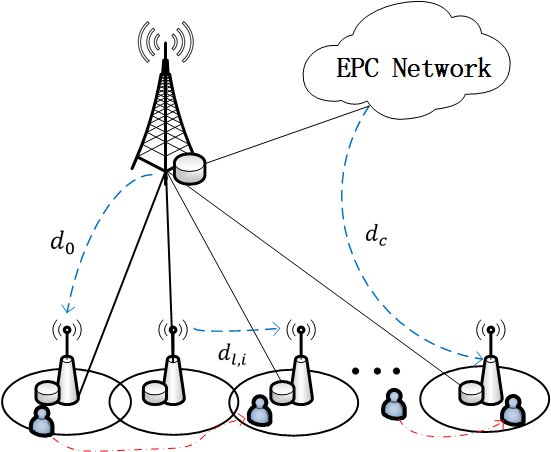
\includegraphics[scale=0.5]{fig2.png}}
 \caption{Delay Model.}
 \label{fig 2}
\end{figure}

home SBS cache hits do not need transmission delay. The transmission delay of MBS transfering file to home SBS is $d_0=\frac{B}{r_{FH}}$.

SBS $l$ share file to home SBS i will cause different transmission delay depending on the hops number h, which can be denoted by $d_{l,i}=h\frac{B}{r_{FH}}$.

Retrieving files from the EPC network through the backhaul link generally results in a large transmission delay $d_c=\frac{B}{r_{BH}}$.

So, given a cache placement matrix $\mathbf{X}$, we can get the average transmission delay of user \emph{u} in cell \emph{i} requesting file \emph{j} as,
\begin{equation}
D_{u,i,j}=(1-x_{i,j})(x_{o,j}d_0+\frac{1-x_{o,j}}{K-2}\sum_{l\in S\setminus{\{o,i\}}}x_{l,j}d_{l,i})+c_{i,j}d_c
\end{equation}
where $c_{i,j}= \prod_{l\in S}1-x_{i,j}$, which means file $j$ is not storaged in RAN.

The QoS guarantee parameter can be expressed as,
\begin{equation}
\theta_{u,i,j}=-\lim_{D_{max}\to \infty}\frac{\log(Pr\{D(\infty)>D_{max}\})}{D_{max}-\sum_i d_i}
\end{equation}
\section{Mobility-aware Cachig Strategy with Effective Capacity}
Here, we first explore the impact of user mobility on file popularity of different base stations. Then, we cast the cache placement optimization problem, which is aimed at maximizing the system effective capacity.
Mobility-aware content request probability: When a user with an incomplete download session of content $j$ arrives at cell $k$, part of the file, $B_{k,j}$, has been downloaded already; hence the user only needs to download the rest of the content $j$. For simplicity, we assume the maximum bandwidth of G [MB/s] of each BS is shared equally among the associated users of that BS. Thus, the bandwidth allocated to each user connecting to BS $l$is given by $r_l=\frac{G}{U_l}$.

Since each content file has B MB, the time needed to completely download one content at cell l is $t_l=B/r_l$.
However, the sojourn time that user stays in cell $l$ is subject to exponential distribution, so the probability of the user completing the download when leaving the cell l can be inferred using the Cumulative Distribution Function $F(\tau,\mu_l)$ as,
\begin{equation}
q_{l,j}=Pr(\tau<t_l-\frac{B_{l,j}}{r_l})=AAAAAAAAAA
\end{equation}
Then,the file requested probability $p_(i,j)$ for content $j$ at cell $i$ is,
\begin{equation}
\mathbf{p_{i,j}}=
\begin{cases}
p_{i,j}+\lambda\sum_{l\neq i}q_{l,j}p_{l,j},  & i=0\\
p_{i,j}+(1-\lambda)\sum_{l\neq i}q_{l,j}p_{l,j}T_{l,j}, & i\in S\setminus 0
\end{cases}
\end{equation}
Where $p_(i,j)$ is the prior popularity of file $j$ at cell $i$ and $T_(l,i)$ is the transition probability from cell $l$ to $i$. And $\lambda\in(0,1)$ is cosntant determined empirically, controlling the tendency of the file cache hierarchy. A larger $\lambda$ factor will make files with higher mobile strength tend to be cached in the MBS cache, voiding cache misses caused by frequent handovers among SBS. Conversely, a smaller $\lambda$ factor will make the file tend to be cached in the SBS cache closer to the user, minimizing the transmission delay.
\section{Problem Formulation}
Based on the system model and effective capacity theory previously mentioned, the effective capacity achieved by user $u$ in cell $i$ can be expressed by the following formulation:
\begin{equation}
EC_{u,i}=\sum_j\mathbf{p_{i,j}}(-\frac{1}{\theta_{u,i,j}T}\log Ee^{-\theta_{u,i,j}Tr_i})
\end{equation}
The problem can be formulated as follows with the purpose of maximizing the sum effective capacity of the whole system.
\begin{equation}
 \begin{aligned}
   & {max}\ \sum_u\sum_iEC_{u,i}\\
   & s.t. \quad\sum Bx_{i,j}<C_i\\
   & \qquad \ x_{i,j}\in\{0,1\}
 \end{aligned}
\end{equation}
Obviously, the optimal problem is a Mixed-Integer Nonlinear Programming (MINLP) and it is highly complicated to find the global optimization solution. In next section, the Genetic Algorithm (GA) is adopted to get a sub-optimal solution.
\section{The Solution of Optimal Problem}
Genetic Algorithm [5] is adaptive heuristic search algorithm premised on the evolutionary ideas of natural selection and genetic. The basic concept of GA is designed to simulate processes in natural system necessary for evolution, specifically those that follow the principles first laid down by Charles Darwin of survival of the fittest. As such they represent an intelligent exploitation of a random search within a defined search space to solve a problem. The processes of GA include coding, colony initialization, initialization, crossover and mutation.

The GA maintains a population of possible cache placement solutions. A solution corresponds to a chromosome which is an encoded representation of the cache placement of all the SBS and MBS.

\subsection{Coding}
We choose the linear structure coding method, in which a chromosome represents a feasible solution of the cache allocation problem. There are $N(K+1)$ elements in each chromosome as shown in fig3; each element records the allocation information in the corresponding cache placement matrix $\mathbf{X}$.
\begin{figure}[htbp]
 \centerline{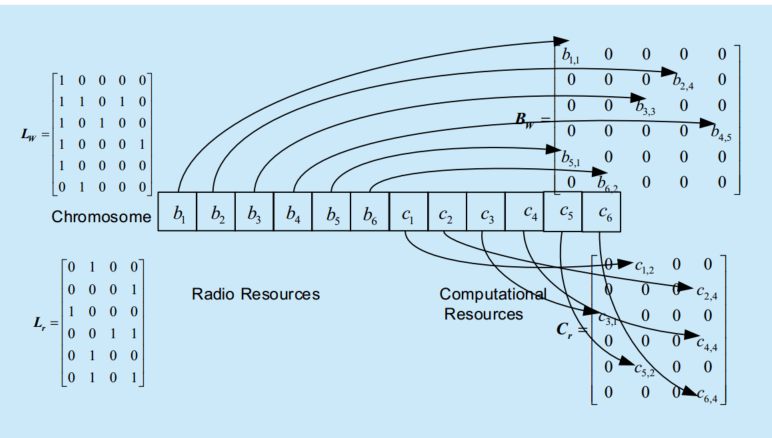
\includegraphics[scale=0.5]{fig3.png}}
 \caption{Coding of Genetic Algorithm.}
 \label{fig 3}
\end{figure}

\subsection{Colony initialization}
We generate Zg chromosomes with $\frac{\sum_{i=0}^KC_i}{NB}$ number of 1 randomly distributed so as to satisfy the cache capacity constrain.
\subsection{Fitness function}
Fitness function is the system optimal function defined in equation (1).
\subsection{Selection}
The chromosomes in the colony are ranked, then the first $x\%$ (Elite selection ratio) is selected and the remains are selected at random. This strategy can guarantee that the genetic algorithm converges to the global optimal solution.
\subsection{Crossever}
For two chromosomes to be mated which are chosen with crossover probability Pc, exchange the each corresponding element with probability $Ps$ (crossover ratio).
\subsection{Mutation}
For each chromosome chosen with mutation probability Pm, replace each element with a random value with probability Pb (mutate ratio).
\subsection{Algorithm process}
\begin{enumerate}[step 1]
\item Initialize colony.
\item Evaluate the individual in colony using fitness function, if the evolutionary generation reaches to the terminal generation then jump to step 4, otherwise continue.
\item Generate the new colony using selection, crossover and mutate operator, then jump to step 2.
\item Get the cache placement matrix through the best individual generated by genetic algorithm.
\item Deliver files to each BS accroding to the cache placement matrix. Cache placement in this cycle is over.
\end{enumerate}
\section{Performance Evaluation}
In this section, we use computer simulation methods to evaluate the performance of the mobility-aware proactive caching placement scheme for heterogeneous ultra density networks. We simulated a heterogeneous ultra density network depicted in Fig1, where the MBS is located in the center and 16 SBSs are uniformly deployed in the network. Moreover, we devided the macrocell into 4 clusters, and each cluster consists of 4 SBSs. Additionally, we consider a wrap-around network layout such that when a user moves out of the network on one side, it comes back in on the opposite side w.r.t. the origin. There several users in the network and the initial location of the users is random, following a uniform distribution. We assume that the files users request can be modeled as the Zipf distribution. The request probability of file $f_j$ is
$$p_j=\frac{1/j^\gamma}{\sum_{i=1}^N 1/j^\gamma}, \quad \forall j\in F$$
where $\gamma\in \{0.3,1.3\}$ is the skewness reflecting the concentration of the popularity distribution among users. Moreover, we consider a library of $N=200$ files, each of size$B=50$MB. The popularities of the files at each BS are generated randomly simulating different file preferences in different regions. The backhaul rate is set to $r_{}= 1000Mbps$ and the fronthaul rate$ r_{FH=}600Mbps$.

The paremeter of genetic algorithm are set as Table\ref{tab1} shown.
\begin{table}[htbp]
 \caption{Simulation Parameters}
 \begin{center}
  \begin{tabular}{|l|l|}
   \hline
   Parameters                     & Value              \\\hline
   Colony size $Z_g$              & 50                 \\ \hline
   Terminal generation number     & 100                \\\hline
   Crossover probability $P_c$    & 0.75               \\ \hline
   Aberrance probability $P_m$    & 0.02               \\\hline
   Reserve ratio x\%              & 25\%               \\\hline
   Crossover ratio $P_s$          & 0.5                \\\hline
   Mutate ratio $P_b$             & 0.05               \\\hline
  \end{tabular}
  \label{tab1}
 \end{center}
\end{table}

We compare the performance of our optimal caching scheme with MPC (most popular caching) schemes, which uses global static content popularity and each BS stores the most populay files until its cache is full.
\subsection{Capacity Based System Tthroughput Performance}
Fig.\ref{fig 4} illustrate the performance of our proposed scheme where we set $\gamma=0.7$ and $\mu=4$. Fig.\ref{fig 4} shows the effective capacity based system throughput when the num of users varies in the network. Obviously we see that as the number of user increases, the system throughout improves and the mobility-aware caching strategie always outperforms the MPC strategy. This is because that files cached in the SBS and MBS changes according to users’ location and preference. Hence, it can match the user request better and reduce the transmition delay.
\begin{figure}[htbp]
 \centerline{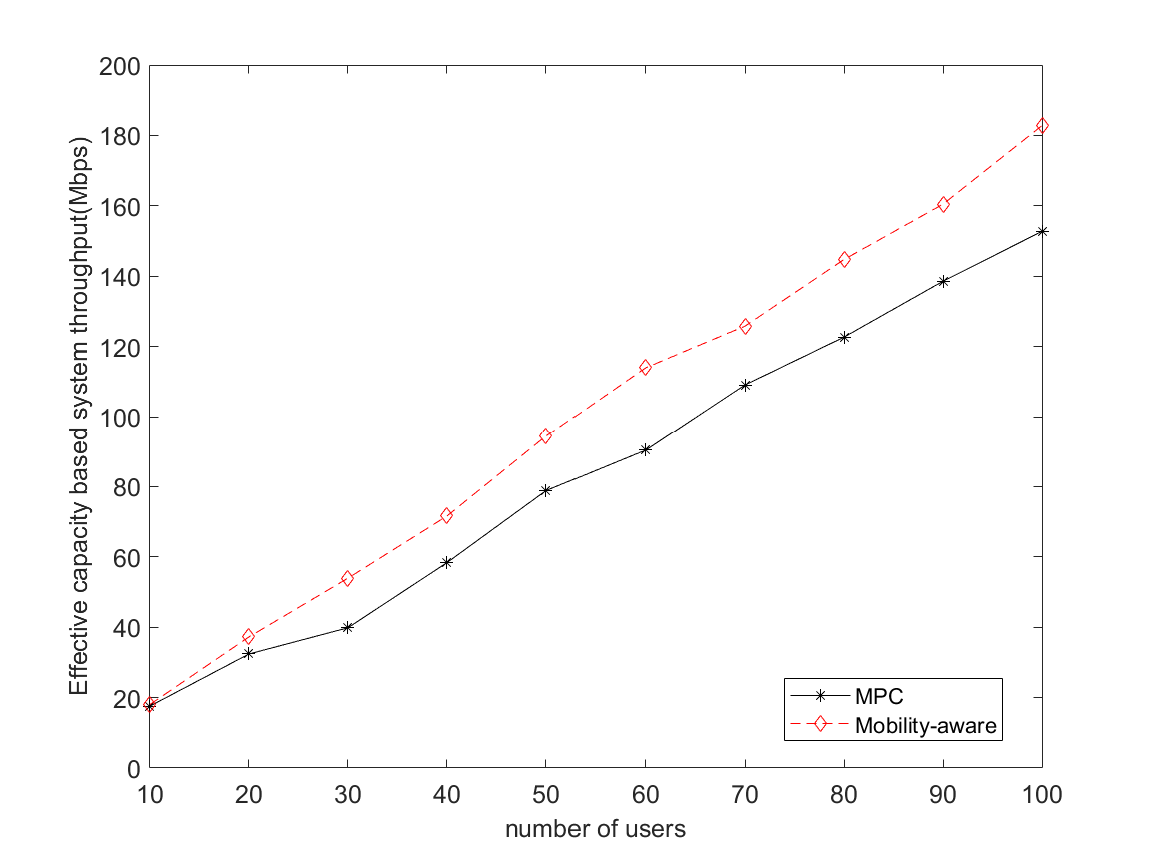
\includegraphics[scale=0.35]{fig4.png}}
 \caption{Fig4.}
 \label{fig 4}
\end{figure}

Fig.\ref{fig 5}investigate the relationship between cache size and system throghput. As shown in Fig.\ref{fig 5}, with the total cache size increases, the effective capacity based system throughput gains at the same time. It demonstrates the fact that expense of storage can alleviate the shortage of backhaul bandwidth and improve the data rate that a user achieves. The more contents BSs cache, the more chances users can get the contents in RAN so that they can be served immediately.
\begin{figure}[htbp]
 \centerline{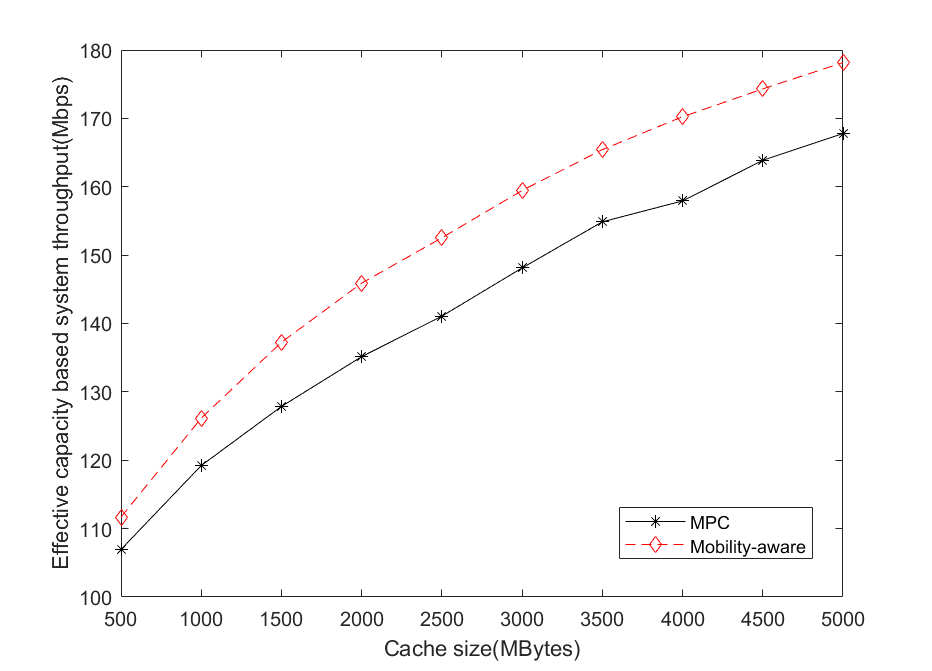
\includegraphics[scale=0.3]{fig5.png}}
 \caption{Fig5.}
 \label{fig 5}
\end{figure}
\subsection{Cache Hit Ratio Performance}
Fig.\ref{fig 6} display the impact of file populatity distribution parameter $\gamma$ on the cache hit ratio. In this simulation, user number is set to 70. As the figure shows, when $\gamma$is small, both two caching strategy have low cache hit ratio. Because in this case, all files are nearly equally likely to be requested but the storage capacity of BS is limited. But mobility-aware caching strategy still achieves superior performance than MPC. When $\gamma$ becomes larger, the requests are more concentrated among some popular files. Therefore, these files are more likely to be cached in most of the SBS resulting in hitting more user requests. Hence the caching hit ratio of mobility-aware and MPC both improve notably.
\begin{figure}[htbp]
 \centerline{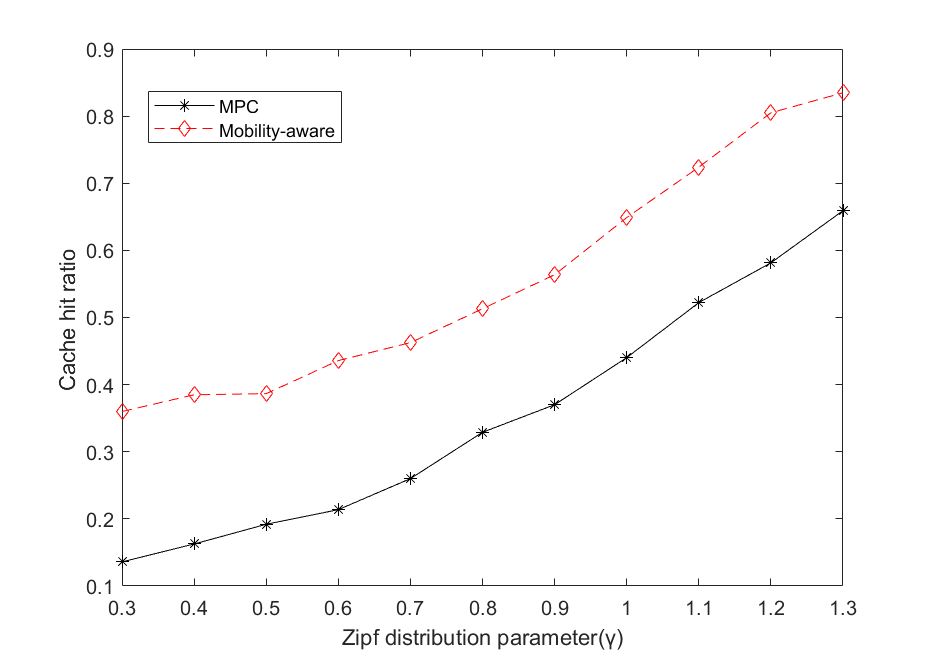
\includegraphics[scale=0.3]{fig6.png}}
 \caption{Fig6.}
 \label{fig 6}
\end{figure}
\section{Conclusion}

\begin{algorithm}[htb]
 \caption{Admission Control.}
 \label{alg:admission}
 \begin{algorithmic}[1] %这个1 表示每一行都显示数字
  \REQUIRE ~~\\ %算法的输入参数:Input
  Admission control vector $\mathbf{A}$ with $a_m=1, \forall \emph{m}\in \mathbf{M}$.
  \ENSURE ~~\\ %算法的输出:Output
  Admission control vector $\mathbf{A}$.
  \FORALL{$\mathrm C_q\in \mathbf{C}$}
  \WHILE {$\left|\mathrm{C_q}\right|>N$}
  \IF{$\mathbf{L}\cap\mathrm{C_q}\neq \emptyset$}
  \STATE $v_m=arg \underset{v_m\in \mathbf{L}\cap\mathrm{C_q}}{max} \left|\mathrm{C_q}\right|$;
  \ELSE
  \STATE $v_m=arg \underset{v_m\in \mathbf{H}\cap\mathrm{C_q}}{max} \left|\mathrm{C_q}\right|$;
  \ENDIF
  \STATE $a_m=0$;
  \STATE $\mathrm{C_q}\leftarrow \mathrm{C_q}\setminus v_m, \forall\mathrm{C_q}\in\mathbf{C^m}$
  \STATE $\left|\mathrm{C_q}\right|--$
  \ENDWHILE
  \STATE Employ greedy algorithm to allocate RBs.
  \ENDFOR
  \STATE Remove added edges and regain some RBs for the corresponding vertices.
 \end{algorithmic}
\end{algorithm}
$\sum_{l=1}^L a_{l,n}^{(c)}>M_N$
In this paper, we proposed a new mobility-aware proactive caching strategy for heterogeneous ultra-dense network and use the effective capacity to evaluate the effect of transmission delay. We use random jump model and stationary Markov model to describe the mobile pattern of user and amend the popularity at BSs with it. Then, we formulated the optimal content placements problem and solved it by genetic algorithm. Finally, simulation results show that the proposed mobility-aware proactive caching strategy achieves higher throughput and cache hit ratio than MPC strategy while users are moving. This indicates that our proposed caching strategy is a promising way to address the challenge of network densification.
\bibliographystyle{IEEEtran}
\bibliography{reference}
\end{document}
